
Sile koje djeluju na projektil su u letu su aerodinamičke, pogonske sile i 
gravitaciona sila. Ove sile se mogu razložiti po osama kooridnatnog sistema vezanog 
za tijelo. 
\section{Aerodinamičke sile}
Aerodinamička sila je posljedica djelovanja pritiska okolnog fluida na tijelo u pokretu. 
Aerodinamička sila se može razložiti na tri komponente koje su definisane u nastavku:
\begin{itemize}
    \item \textbf{Uzgon}- Uzgon je komponenta rezultantne aerodinamičke sile 
    koja je normalna na relativno kretanje vjetra.
    \item \textbf{Otpor}- Otpor je komponenta rezultantne aerodinamičke sile 
    koja je paralelna relativnom kretanju vjetra.
    \item \textbf{Bočna sila}- Bočna sila je komponenta rezultantne aerodinamičke sile 
    koja je normalna na uzogn i otpor. 
\end{itemize}
Ovdje se posmatraju projektili koji se zakreću da bi skrenuli(skid to turn) i 
kod takvih projektila aerodinamičke sile su date sa:
\begin{equation}
   \text{Otpor} \quad R_x=C_xqS
   \label{eq:aa1}
\end{equation}
\begin{equation}
    \text{Uzgon} \quad R_z=C_zqS
    \label{eq:aa2}
\end{equation}
\begin{equation}
    \text{Bočna sila} \quad R_y=C_yqS
    \label{eq:aa3}
\end{equation}
,gdje su $C_x,C_y$ i $C_z$ aerodinamički koeficijenti, $q$ dinamički pritisak slobodnog strujanaja
u tački daleko od objekta i iznosi $q=\frac{1}{2}\rho v^2$, $S$ je referentna površina i 
$v$ je brzina vazduha, $\rho$ predstavlja atmosferski pritisak.
\\
Treba napomenuti da se aerodinamičke sile i momenti izražavaju bezdimenzionalnim veličinama. 
To se postiže tako što se dogovorom utvrdi da se sila(ili moment) predstavlja svojim odgovarajućim 
aerodinamičkim koeficijentom. Prema tome, $C_x$ potpuno određuje silu otpora i slično vrijedi i 
za ostale koeficijente. \\

U opštem slučaju koeficijenti aerodinamičkih sila su funkcije varijabli stanja pa se može
napisati:
\begin{equation}
    C_x=C_x(\alpha ,\beta, M,q,\delta_v,\delta_P,\delta_e)
\end{equation}
,gdje je $M$ Mahov broj- odnos tekuće brzine i brzine zvuka, $\alpha$ napadni ugao i 
$\beta$ ugao klizanja. Slično tako vrijedi:
\begin{equation}
    C_z=C_z(\alpha ,\beta, M,q,\delta_v,\delta_P,\delta_e)
\end{equation}
Uglovi $\alpha, \beta$ i $\gamma$ su prikazani na slici \ref{fig:angles} i definisani su sa:
\begin{equation}
    \alpha=arctg(w/u)
\end{equation}
\begin{equation}
    \beta=\arcsin(v/v_m)
\end{equation}
\begin{figure}[ht!]
    \centering
    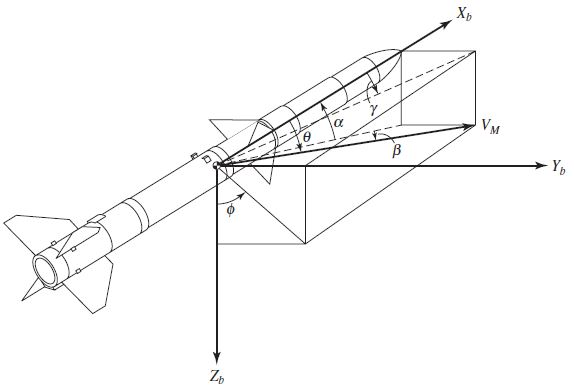
\includegraphics[scale=0.7]{angles.JPG}
    \caption{Ugaone veze}
    \label{fig:angles}
\end{figure}
Razvojem u Taylorov red i odbacivanjem viših članova dobija se aproksimacija 
aerodinamičkih koeficijenata:
\begin{equation}
    C_x=C_{x_0}+C_{x_\alpha}|\alpha|+C_{x_\alpha^2}\alpha^2+C_{x_\beta}|\beta|+
    C_{x_\beta^2}\beta^2+C_{x_\alpha \beta}|\alpha||\beta|
\end{equation}
\begin{equation}
   C_z=C_{z_0}+C_z^{\alpha}{\alpha} + C_z^{\dot{\alpha}} \dot{\alpha}+C_z^q q+C_z^{\delta _v}{\delta _v}
\end{equation}
\begin{equation}
    C_y=C_{y_0}+C_y^{\alpha}{\alpha} + C_y^{\dot{\alpha}} \dot{\alpha}+C_y^q q+C_y^{\delta _v}{\delta _v}
\end{equation}
U datom slučaju aerodinamički koeficijent otpora imaju jednostavniji oblik
\begin{equation}
    C_x=C_{x_0} + C_{x_1}\alpha
\end{equation}
,gdje je $C_{x_0}=\frac{\partial c_x}{\partial \alpha}|_{\alpha=0}$, $C_{x_1}=\frac{\partial c_x}{\partial \alpha}$ 
i slično tako za ostale izvode.\\
Također je važno istaći da su ovi koeficijenti(tj. sile) izražene u \textit{kooridnatnom sistemu vjetra} 
relativnom toku vazduha. Koordinatni sistem vazduha je prikazan na slici \ref{fig:wind}. 
\begin{figure}[ht!]
    \centering
    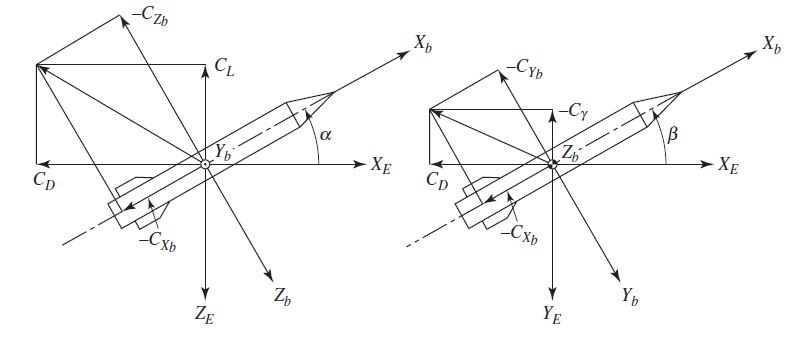
\includegraphics[scale=0.5]{wind.JPG}
    \caption{Veza između sistema tijela i sistema vjetra}
    \label{fig:wind}
\end{figure}
Pošto su jednačinama kretanja tijela sile izražene sistemu tijela, potrebno
je imati transformaciju koja transformiše aerodinamičke sile u sistem tijela i njihova veza je data sa:
\begin{equation}
    \begin{bmatrix}
        C_{x_b}\\
        C_{y_b}\\
        C_{z_b}\\
    \end{bmatrix}=\begin{bmatrix}
        \cos\alpha && -\cos\alpha && \sin\alpha\\
        \sin\beta &&\cos\beta && 0\\
        \sin\alpha\cos\beta && -\sin\alpha\sin\beta && \cos\alpha\\
    \end{bmatrix}\begin{bmatrix}
        -C_x\\
        C_y\\
        -C_z\\
    \end{bmatrix}
\end{equation} Sada se vraćanjem u \ref{eq:aa1},\ref{eq:aa2} i \ref{eq:aa3} mogu odrediti 
aerodinamičke sile koje djeluju na projektil. 
\section{Aerodinamički momenti}
Momenti se mogu podjeliti na momente koji su posljedica aerodinamičkog tereta i 
pogonske sile koja ne djeulje kroz centar gravitacije. Moment koji je posljedica 
rezultantne sile koja ne djeluje na centar kooridnatnog sistema tijela se može 
podjeliti na tri komponente, i to:
\begin{itemize}
    \item \textbf{Moment valjanja} je moment oko lateralne ose($Y_b$) projektila i generisan 
    je od uzgonom i otporom koje djeluju na tijelo. Pozitivan moment je u smjero gore 
    od nosa letjelice 
    
    \item \textbf{Moment propinjanja} je moment oko longitudinalne ose($X_b$) projektila.
    Posljedica je uzogna koji je uzrokovan nekom vrstom elerona. Pozitivan moment propinjanja uzrokuje kretanje nadole 
    desnog krila.
    
    \item \textbf{Moment zakretanja} je moment oko vetikalne ose projektila($Z_b$). Pozitivan moment zakretanja 
    ima za posljedicu da se nos aviona zakrene u desno. 
\end{itemize}
Kvantitativno, momenti su dati sa:
\begin{equation}
    \text{Moment valjanja} \quad L=C_lqSb
    \label{eq:a1}
 \end{equation}
 \begin{equation}
     \text{Moment propinjanja} \quad M=C_mqSc
     \label{eq:a2}
 \end{equation}
 \begin{equation}
     \text{Moment zakretanja} \quad N=C_nqSb
     \label{eq:a3}
 \end{equation}
 ,gdje je $b$ raspon krila, $c$ je razmak između početne i krajnje ivice krila mjerene 
 u smjeru paralelnom toku vazduha, $S$ je površina platforme krila. 
 Isto kao i kod slučaja sa silama, koeficijenti momenata također zavise od više promjenjivljih 
 i potrebno ih je linearizirati. \\
 Linearizirani koeficijenti momenta su:
 \begin{equation}
     C_m=C_m^{\alpha}\alpha +C_m^{\dot{\alpha}}\dot{\alpha } + C_m^q q+C_m^{\delta _v}\delta _v
 \end{equation} 
 ,i koeficijent momenta valjanja:
 \begin{equation}
     C_L = C_l^PP+C_l^QQ+C_l^RR +C_l^\alpha \alpha +C_l^\beta \beta + C_l^{\delta _e} \delta _e +C_l^{\delta _v} \delta _v
     +C_l^{\delta _P} \delta _P
 \end{equation}